\documentclass[12pt,a4paper,final,titlepage,twoside]{article}
\usepackage{MLABdoc}
\fancyhead[L]{{\huge RTC03A}}
\fancyfoot[RE,LO]{\today\hspace{1pt}|  | mlab.cz}

\includeonly{RTC03A.cs.title, RTC03A.cs.assembly}

\begin{document}
%vytvori uvodni stranku
\uvod
% nazev modulu
{RTC03A}
% kratky popis
{hodiny reálného času s funkcí čítače}
%autor/i
{}
%obrazek
{../..//doc/img/pcb.png}
%abstrakt
{Modul obsahuje hodiny reálného času PCF8583, který po přenastavení může fungovat jako čítač signálů až do 20kHz.}
%tabulka
{ }
%obrazek QR kodu
{../../doc/img/RTC03A_QRcode.png}


\section{Popis konstrukce}

\subsection{Zapojení}
%naimportuje schema 
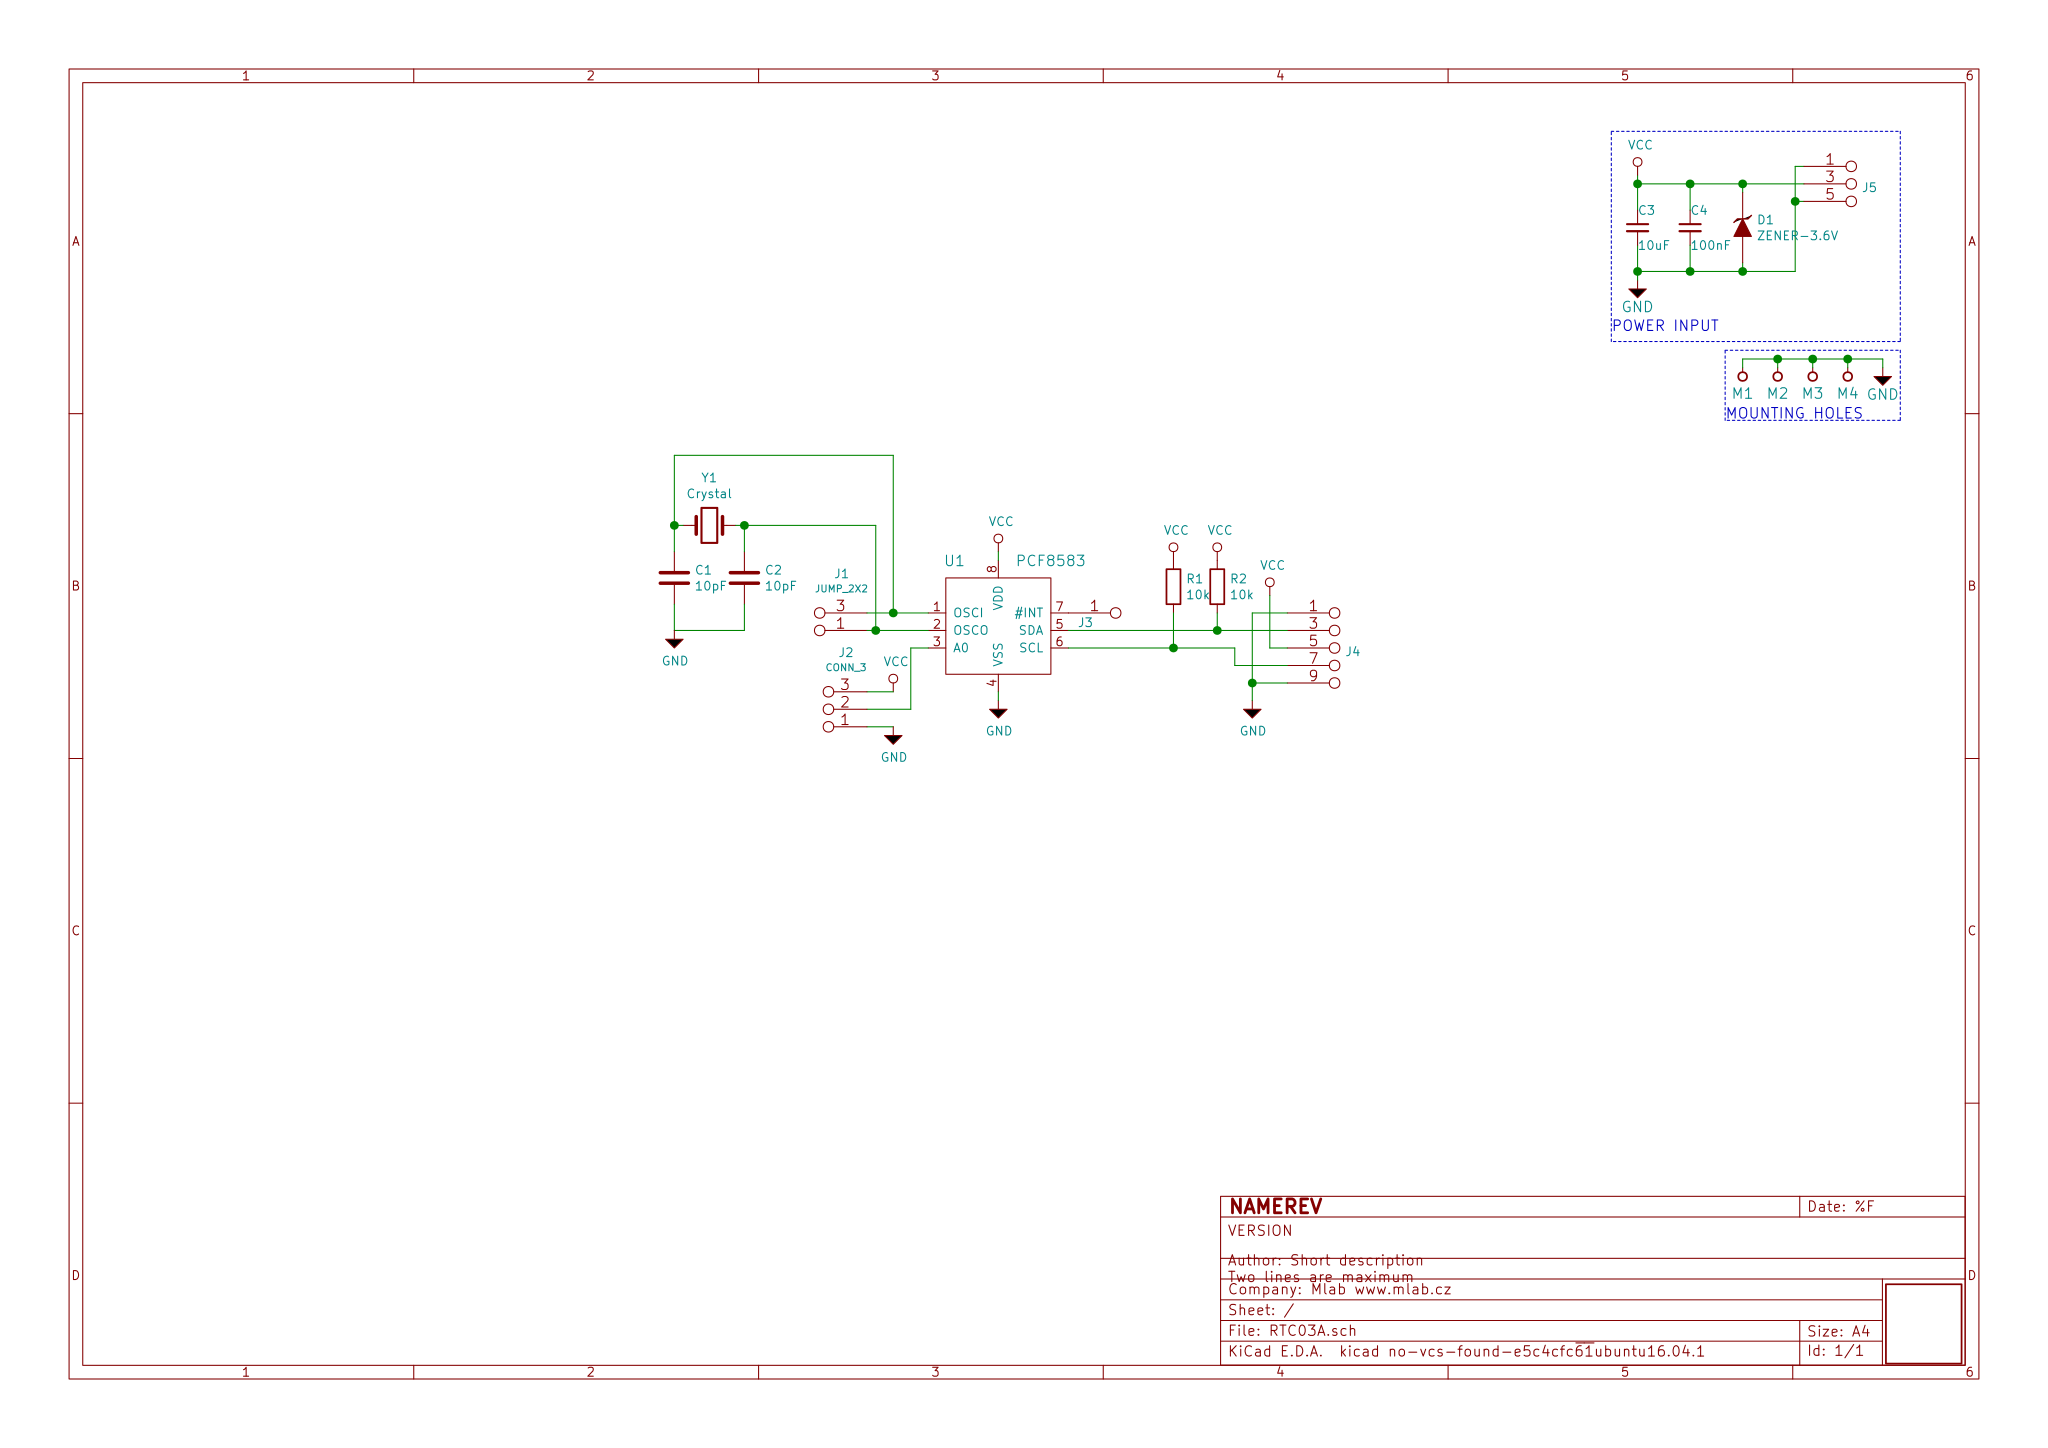
\includepdf[angle=90]{../../hw/sch_pcb/RTC03A.pdf}

\subsection{Odrušení}

\subsection{Mechanická konstrukce}

\section{Výroba a testování}

% totot naimportuje cast, kde jsou osazováky a BOM tabulka
\subsection{Osazení}


\begin{figure}[ht!]
	\centering
	\includegraphics[scale=2]{../../hw/cam_profi/RTC03A-top_cropped.pdf}
	\qquad
	\includegraphics[scale=2]{../../hw/cam_profi/RTC03A-bottom_cropped.pdf}
\end{figure}

\begin{center}
  \begin{tabular}{ | l | l | l | l |}
    \hline
    Označení & Hodnota, typ & Pouzdro & Počet \\ \hline
    \hline
			J1 & JUMP\_2X2 & Straight\_2x02 & 1\\ \hline
			J3 & JUMP\_2x1 & Straight\_2x01 & 1\\ \hline
			D1 & ZENER-5.6V & Diode-MiniMELF\_Standard & 1\\ \hline
			J6 & JUMP2\_2x1 & Straight\_1x02 & 1\\ \hline
			J2 & CONN\_3 & Straight\_1x03 & 1\\ \hline
			C1, C2 & 10pF & C\_0805 & 2\\ \hline
			Y1 & Crystal & Crystal\_HC49-U\_Vertical & 1\\ \hline
			R3, R2, R1 & 10k & SMD-0805 & 3\\ \hline
			U1 & PCF8583 & SO-8 & 1\\ \hline
			J5 & JUMP\_3X2 & Straight\_2x03 & 1\\ \hline
			M1, M2, M3, M4 & HOLE & MountingHole\_3mm & 4\\ \hline
			C4 & 100nF & SMD-0805 & 1\\ \hline
			C3 & 10uF & SMD-0805 & 1\\ \hline
			J4 & JUMP\_5X2 & Straight\_2x05 & 1\\ \hline
	
  \end{tabular}
\end{center}

Krystal $Y1$ a kondenzátory $C1$ a $C2$ jsou volitenlé. Pro režim čítání nejsou potřeba. Krystal je vhodné osadit, pokud použití modulu se předpokládá jako zdroj reálných hodin a interní čítač není dostatečně přesný.
\subsection{Nastavení}

\section{Programové vybavení}


\end{document}